% (c)~2014 Claudio Carboncini - claudio.carboncini@gmail.com
% (c)~2014 Dimitrios Vrettos - d.vrettos@gmail.com
\chapter{Equazioni e disequazioni irrazionali}
\section{Equazioni irrazionali con un solo radicale}

\begin{definizione}
Un'equazione si dice \emph{irrazionale} quando l'incognita compare sotto il segno di radice.
\end{definizione}

Analizziamo le seguenti equazioni: $\sqrt 3\cdot x=x^2-x+2$~~e~~$\sqrt{2x}=x^2-x$.
Notiamo che l'equazione $\sqrt 3\cdot x=x^2-x+2$ è di secondo grado, intera con un coefficiente irrazionale (sotto il segno di radice), ma non è un'equazione irrazionale perché l'incognita non compare sotto la radice.
Nell'equazione $\sqrt{2x}=x^2-x$, invece, il monomio $ 2x $ (contenente l'incognita) compare sotto il segno di radice, pertanto essa è un'equazione irrazionale.
\begin{problema}
Determinare l'area di un triangolo rettangolo $ABC$, retto in $A$, avente perimetro di $24\unit{cm}$ e i cateti che differiscono di $2\unit{cm}$.
\end{problema}

\begin{multicols}{2}
\emph{Dati}:

$2p=24$;

$\overline{AB}-\overline{AC}=2$.

\emph{Obiettivo}:
Area.

% (c) 2013 Claudio Carboncini - claudio.carboncini@gmail.com
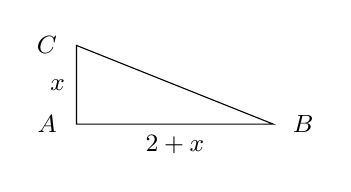
\begin{tikzpicture}[x=10mm,y=10mm,font=\small]
  \draw (1,1) -- (1,2) -- (3.5,1) -- cycle;
  \node [label={[name=label node]left:$C$}] at (1,2) {};
  \node [label={[name=label node]right:$B$}] at (3.5,1) {};
  \node [label={[name=label node]left:$A$}] at (1,1) {};
  \node [label={[name=label node]left:$x$}] at (1.1,1.5) {};
  \node [label={[name=label node]below:$2+x$}] at (2.25,1.1) {};
  
\end{tikzpicture}

\end{multicols}

\begin{soluzione}
${\Area}=\frac{\overline{AB}\cdot \overline{AC}} 2$; dobbiamo quindi determinare i cateti. Poniamo $\overline{AC}=x$ con $x>0$ quindi $\overline{AB}=2+x$ e sfruttiamo l'informazione relativa al perimetro per determinare l'equazione risolvente $\overline{AB}+\overline{AC}+\overline{BC}=24$.

Applicando il teorema di Pitagora si ricava $\overline{BC}=\sqrt{x^2+(2+x)^2}=\sqrt{2x^2+4x+4}$ e dunque otteniamo l'equazione risolvente $2x+2+\sqrt{2x^2+4x+4}=24$ in cui l'incognita compare sotto il segno di radice. Vedremo nel seguito come risolvere un'equazione di questo tipo.
\end{soluzione}

\subsection{Equazioni irrazionali con la radice di indice pari}

Ricordiamo che l'espressione irrazionale $E=\sqrt[n]{f(x)}$ con $n$ pari maggiore di $1$ ha significato per tutti i valori di $x$ che rendono non negativo il radicando, pertanto l'insieme soluzione di un'equazione irrazionale in cui compaiono uno o più radicali di indice pari sarà un sottoinsieme del dominio o insieme di definizione del radicale (condizione di realtà del radicale).

Per esempio, nell'equazione $\sqrt{2x}=x^2-x$ si ha che il dominio $\Dom$ del radicale è dato da $x\ge 0$, cioè $\Dom=\insR^{+}\cup \{0\}$. Pertanto l'insieme delle soluzioni è un sottoinsieme di tale dominio, cioè $\IS\subseteq \Dom$. Nessun numero negativo potrà essere soluzione dell'equazione, altrimenti il radicale non sarebbe un numero reale.
Inoltre, poiché l'espressione irrazionale $\sqrt[n]{f(x)}$ nel suo $\ID$ è positiva o nulla (per definizione), l'equazione $\sqrt{2x}=x^2-x$ potrà verificarsi solo se il secondo membro sarà non negativo (condizione di concordanza del segno).

Quando abbiamo un'equazione nella quale l'incognita compare sotto una radice di indice $n$ pari possiamo elevare alla potenza $n$ entrambi i membri dell'equazione eliminando la radice. Tuttavia, l'equazione ottenuta non sempre è equivalente a quella data, ossia non sempre ha le stesse soluzioni dell'equazione data (in genere ne ha di più).

\begin{exrig}
\begin{esempio}
Risolvere la seguente equazione irrazionale $ \sqrt{x+2}=x $.

Elevando al quadrato si ha $x+2=x^2$ da cui $x^2-x-2=0$. Risolvendo questa equazione di secondo grado otteniamo le soluzioni $x_1=-1$~~e~~$x_2=2$. Tuttavia, sostituendo questi valori di $x$ nell'equazione irrazionale di partenza si ha:
\begin{itemize}
\item per $x=-1 \:\Rightarrow\: \sqrt{-1+2}=-1 \:\Rightarrow\: \sqrt 1=-1$ che è falsa, pertanto $x=-1$ non può essere soluzione;
\item per $x=2 \:\Rightarrow\: \sqrt{2+2}=2 \:\Rightarrow\: \sqrt 4=2$ che è vera, pertanto $x=2$ è l'unica soluzione.
\end{itemize}

Quindi l'insieme soluzione dell'equazione data è $\IS=\{2\}$.
\end{esempio}
\end{exrig}

\conclusione Per risolvere un'equazione irrazionale con indice pari possiamo allora elevare alla potenza pari della radice i due membri dell'equazione, risolvere l'equazione che si ottiene e verificare se le soluzioni trovate sono accettabili.

Possiamo però procedere in un altro modo: l'insieme soluzione dell'equazione irrazionale $\sqrt[n]{f(x)}=g(x)$ con $n$ pari non nullo sarà un sottoinsieme dell'insieme in cui sono contemporaneamente vere le condizioni 
\[\left\{\begin{array}{l}{f(x)\ge 0}\\{g(x)\ge 0}\end{array}\right..\]

\begin{exrig}
\begin{esempio}
Risolvere le seguenti equazioni irrazionali con radice di indice pari.
\begin{itemize}
\item $\sqrt{x+2}=x$.

La soluzione si ottiene risolvendo 
\[\left\{\begin{array}{l}x+2\ge 0 \\x\ge 0\\x+2=x^2 \end{array}\right.\Rightarrow \left\{\begin{array}{l}x\ge 0\\x+2=x^2 \end{array}\right..\]

Le soluzioni dell'equazione $x^2-x-2=0$ sono $x_1=-1\vee x_2=2$, ma l'unica accettabile è $x=2$ (per la condizione $x\ge 0$).

\item $\sqrt{5-2x}=x-1$.

Elevo ambo i membri al quadrato, ottengo $5-2x=x^2-2x+1 \:\Rightarrow\: x^2=4 \:\Rightarrow\: x_{1\text{,}2}=\pm 2$,
sostituisco $x=-2$ ottengo $\sqrt{5-2\cdot (-2)}=-2-1 \:\Rightarrow\: \sqrt 9=-3$ falso, quindi $x=-2$ non è accettabile;
sostituisco $x=+2$ ottengo $\sqrt{5-2\cdot 2}=2-1 \:\Rightarrow\: \sqrt 1=1$ vero, quindi $x=+2$ è l'unica soluzione dell'equazione data.

Arrivo allo stesso risultato ponendo le condizioni 
\[\left\{\begin{array}{l}5-2x\ge 0 \\x\ge 1\end{array}\right.\Rightarrow \left\{\begin{array}{l}x\le \frac 5 2\\x\ge 1\end{array}\right.\]
che indica l'intervallo $1\le x\le \frac 5 2$. La soluzione $x=-2$ non è accettabile in quando non è compresa tra $1$ e $\frac 5 2$, mentre la soluzione $x=+2$ è invece accettabile.

\item $\sqrt{2x}=x^2-x$.

Determiniamo l'insieme in cui cercare le soluzioni dell'equazione 
\[\left\{\begin{array}{l}{2x\ge 0}\\{x^2-x\ge 0}\end{array}\right.
\Rightarrow
\left\{\begin{array}{l}{2x\ge 0}\\{x(x-1)\ge 0}\end{array}\right.
\]
con soluzione $x=0\vee x\ge 1$.
Rendiamo razionale l'equazione elevando ambo i membri al quadrato: 
\[\left(\sqrt{2x}\right)^2=\left(x^2-x\right)^2\quad\Rightarrow\quad 2x=x^4-2x^3+x^2.\]
Risolviamo l'equazione ottenuta: 
\[x^4-2x^3+x^2-2x=0\quad\Rightarrow\quad x\cdot \left(x^2+1\right)\cdot (x-2)=0\quad\Rightarrow\quad x=0\;\vee\; x=2.\]

Confrontiamo le soluzioni ottenute con le condizioni $x=0\;\vee\; x\ge 1$. Poiché entrambe le soluzioni verificano queste condizioni si ha che $\IS=\{0\text{, }2\}$.
\end{itemize}
\end{esempio}
\end{exrig}

\subsection{Equazioni irrazionali con la radice di indice dispari}

L'espressione irrazionale $E=\sqrt[n]{f(x)}$ con $n$ dispari è definita per tutti i valori reali per cui è definito il radicando, quindi l'equazione irrazionale $\sqrt[n]{f(x)}=g(x)$ è equivalente a quella che si ottiene elevando ad $n$ entrambi i membri dell'equazione: $f(x)=g^n(x)$.

\begin{exrig}
\begin{esempio}
Risolvere le seguenti equazioni irrazionali con radice di indice dispari.
\begin{itemize}
\item $\sqrt[3]{x-2}=\frac 1 2$.

Elevando al cubo si ha $x-2=\frac 1 8\ \:\Rightarrow\: \ x=2+\frac 1 8\ \:\Rightarrow\: \ x=\frac{17} 8$.

\item $\sqrt[3]{-3x^2+3x+1}=x$.

Elevando al cubo si ha $-3x^2+3x+1=x^3\:\Rightarrow\: (x-1)^3=0\:\Rightarrow\: x-1=0\:\Rightarrow\: x=1$.

\item $\sqrt[3]{\frac x{2x+3}}=\frac{2-5x} 4$.

Il dominio del radicando è l'insieme $\Dom=\left\{x\in \insR\mid x\neq -\frac 3 2\right\}$. Per risolvere l'equazione elevo primo e secondo membro al cubo, ottenendo l'equazione $\frac x{2x+3}=\left(\frac{2-5x} 4\right)^3$, la cui risoluzione richiede la risoluzione di un'equazione di quarto grado che non svolgiamo.

\item $ \sqrt[3]{\frac 1 x}=\frac{4x+x^2}{3-x}$.

Le condizioni di esistenza sono: $x\neq 0\;\wedge\; x\neq 3$. Elevando al cubo si ottiene l'equazione risolvente che non svolgeremo.
\end{itemize}
\end{esempio}
\end{exrig}

\ovalbox{\risolvii \ref{ese:8.1}, \ref{ese:8.2}, \ref{ese:8.3}, \ref{ese:8.4}, \ref{ese:8.5}, \ref{ese:8.6}, \ref{ese:8.7}, \ref{ese:8.8}, \ref{ese:8.9}}

\section{Equazioni con più radicali}

Non potendo stabilire una forma canonica, procederemo mediante esempi al fine di acquisire un metodo risolutivo a seconda dei casi che si possono presentare.

\begin{exrig}
\begin{esempio}
Risolvere la seguente equazione irrazionale $\sqrt{2-\frac 1 x}=\sqrt x$.

Osserviamo subito che i due membri, nell'insieme in cui entrambi hanno significato, sono positivi.
Determiniamo quindi l'insieme in cui cercare le soluzioni: 
\[\left\{\begin{array}{l}{2-\frac 1 x\ge 0}\\{x\ge 0}\end{array}\right..\]

Risolvendo le due disequazioni otteniamo 
\[\left\{\begin{array}{l}x<0\vee x\ge \frac 1 2\\{x\ge 0}\end{array}\right.\Rightarrow\: x\ge \frac 1 2.\]

Ora eleviamo al quadrato entrambi i membri dell'equazione e otteniamo $2-\frac 1 x=x$, da cui si ha $x_1=x_2=1$ che è accettabile in quanto maggiore di $\frac 1 2$.
\end{esempio}
\begin{esempio}
Risolvere la seguente equazione irrazionale $\sqrt{x+3}-\sqrt[3]{2x^2+6x}=0$.

Separiamo i due radicali $\sqrt{x+3}=\sqrt[3]{2x^2+6x}$.

Affinché i due membri dell'equazione siano positivi dobbiamo porre la condizione di positività anche al radicando del radicale cubico: 
\[\left\{\begin{array}{l}{x+3\ge 0}\\{2x^2+6x\ge 0}\end{array}\right.\Rightarrow\: x=-3\;\vee\; x\ge 0.\]

Per risolvere l'equazione occorre avere radici con lo stesso indice. Il minimo comune indice è $6$, perciò si ha $\sqrt[6]{(x+3)^3}=\sqrt[6]{\left(2x^2+6x\right)^2}$. Ed elevando alla sesta potenza si ottiene
\[(x+3)^3=\left(2x^2+6x\right)^2 \Rightarrow (x+3)^3-\left(2x^2+6x\right)^2=0 \Rightarrow (x+3)^3-[2x(x+3)]^2=0.\]
%\begin{align*}
%&(x+3)^3=\left(2x^2+6x\right)^2\\
%\Rightarrow & (x+3)^3-\left(2x^2+6x\right)^2=0\\
%\Rightarrow & (x+3)^3-[2x(x+3)]^2=0.
%\end{align*}
Raccogliendo a fattore comune si ha: $(x+3)^2\cdot \left(x+3-4x^2\right)=0$.

Per la legge di annullamento del prodotto abbiamo 
\[\begin{array}{l}(x+3)^2=0\:\Rightarrow\: x+3=0\:\Rightarrow\: x=-3~\text{ e} \\-4x^2+x+3=0\:\Rightarrow\:x_1=-\frac 3 4\;\vee\; x_2=1.\end{array}\]
%\[(x+3)^2=0\:\Rightarrow\: x+3=0\:\Rightarrow\: x=-3\] e 
%\[-4x^2+x+3=0\:\Rightarrow\:x_1=-\frac 3 4\;\vee\; x_2=1.\]

Le soluzioni che verificano le condizioni $x=-3\;\vee\; x\ge 0$ sono $x_1=-3$~~e~~$x_2=1$.
\end{esempio}
\begin{esempio}
Risolvere la seguente equazione irrazionale $\sqrt x+\sqrt{x^3+2x-1}=0$.

Separiamo i due radicali $\sqrt x=-\sqrt{x^3+2x-1}$; osserviamo che i due membri nell'insieme in cui sono definiti sono di segno opposto e dunque l'uguaglianza sarà vera solo nel caso in cui entrambi si annullino.

Il primo membro si annulla solo per $x=0$ che non annulla il secondo membro, pertanto l'equazione non ha soluzioni.
\end{esempio}
\begin{esempio}
Risolvere la seguente equazione irrazionale $-\sqrt{x^2+3x}+\sqrt{2x+2}=0$.

Portiamo la radice con il segno meno a secondo membro, in modo da avere due radici positive:
$\sqrt{2x+2}=\sqrt{x^2+3x}$. Poniamo le condizione sull'accettabilità della soluzione:

\begin{equation*}
\left\{\begin{array}{l}{2x+2\ge 0}\\{x^2+3x\ge 0}\end{array}\right. \Rightarrow \left\{\begin{array}{l}{x\ge -1}\\{x\le -3\vee x\ge 0}\end{array}\right.\Rightarrow\: x\ge 0.
\end{equation*}

Eleviamo al quadrato i due membri dell'equazione 
\[2x+2=x^2+3x\:\Rightarrow\: x^2+x-2=0.\]
Le soluzioni sono $x_1=-2$ e $x_2=1$. Di queste solo $x=1$ soddisfa le condizioni di accettabilità.
\end{esempio}

\begin{esempio}
Risolvere la seguente equazione irrazionale $\sqrt{x+7}-\sqrt{x-1}=2$.

In questo esempio ci sono altri termini oltre i due radicali.

Spostiamo dopo l'uguale il radicale negativo in modo che sia a destra sia a sinistra i termini siano positivi: $\sqrt{x+7}=\sqrt{x-1}+2$.

Poniamo le condizioni sull'accettabilità delle soluzioni: \[ \left\{\begin{array}{l}{x+7\ge 0}\\{x-1\ge 0}\end{array}\right.\Rightarrow \left\{\begin{array}{l}{x\ge -7}\\{x\ge 1}\end{array}\right.\Rightarrow\: x\ge 1. \]

Elevando l'equazione al quadrato si ha: $x+7=4+4\sqrt{x-1}+x-1 \:\Rightarrow\: 4\sqrt{x-1}=4 \:\Rightarrow\: \sqrt{x-1}=1$.

Eleviamo nuovamente al quadrato $\sqrt{x-1}=1$ ottenendo $x-1=1\:\Rightarrow\: x=2$, che è accettabile.
\end{esempio}

\begin{esempio}
Risolvere la seguente equazione irrazionale $\sqrt{x^2+1}-\sqrt{1-4x}=x$.

Per prima cosa porto al secondo membro il radicale che ha il segno negativo, in modo che diventi positivo $\sqrt{x^2+1}=\sqrt{1-4x}+x$.

In questo caso risulta problematico risolvere il sistema con tutte le condizioni di accettabilità, perché bisognerebbe risolvere anche la disequazione irrazionale $\sqrt{1-4x}+x\ge 0$.
Ci limiteremo allora a risolvere l'equazione e poi verificarne le soluzioni.

Elevo al quadrato ambo i membri dell'equazione: $x^2+1=1-4x+x^2+2x\sqrt{1-4x}$.

Semplificando si ha $x(2-\sqrt{1-4x})=0$. Una soluzione è $x=0$, la seconda soluzione si ottiene da $2-\sqrt{1-4x}=0\:\Rightarrow\: 2=\sqrt{1-4x}$. Elevando al quadrato si ha $4=1-4x\:\Rightarrow\: x=-\frac 3 4$.

Verifichiamo ora le soluzioni. Per $x=0$ si ha $\sqrt{(0)^2+1}=\sqrt{1-4\cdot (0)}+0\:\Rightarrow\: 1=1$ soluzione accettabile. Per $x=-\frac 3 4$ si ha $\sqrt{\left(-\frac 3 4\right)^2+1}=\sqrt{1-4\cdot\left(-\frac 3 4\right)}-\frac 3 4\:\Rightarrow\:\frac 5 4=\frac 5 4$ e anche questa è una soluzione accettabile.
\end{esempio}
\end{exrig}
\ovalbox{\risolvii \ref{ese:8.10}, \ref{ese:8.11}, \ref{ese:8.12}, \ref{ese:8.13}, \ref{ese:8.14}, \ref{ese:8.15}, \ref{ese:8.16}, \ref{ese:8.17}, \ref{ese:8.18}}

\section{Disequazioni irrazionali}

Concludiamo con un cenno alle disequazioni irrazionali, nelle quali l'incognita compare sotto radice. Esaminiamo il caso in cui l'incognita è sotto radice quadrata e in cui la disequazione presenta una sola radice. Qualunque sia la disequazione di partenza, ci si può sempre ricondurre ai seguenti due casi.

\paragraph{Primo caso:} disequazioni nella forma: $\sqrt{f(x)}>g(x)$.

Questa disequazione si può ricondurre allo studio di una coppia di sistemi di disequazioni. Infatti distinguiamo due casi a seconda del segno di $g(x)$.

\begin{itemize*}
\item Se $ g(x)<0 $ la disequazione è sicuramente verificata, in quanto al primo membro c'è una quantità sicuramente positiva in quanto radice quadrata, sotto condizione di esistenza del radicando $f(x)\ge 0$. Pertanto, il primo sistema è: 
\[\left\{\begin{array}{l}{g(x)<0}\\{f(x)\ge 0}\end{array}\right..\]
\item Se $g(x)\ge 0$, dopo aver posto la condizione di esistenza del radicale $f(x)\ge 0$ si possono elevare al quadrato i due membri dell'equazione, in quanto entrambi positivi. Si ottiene il sistema 
\[\left\{\begin{array}{l}g(x)\ge 0\\f(x)\ge 0 \\f(x)>\left[g(x)\right]^2 \end{array}\right..\]
La seconda disequazione del sistema si può eliminare in quanto la prima e la terza disequazione implicano automaticamente che $f(x)>0$.
\end{itemize*}

In definitiva:
\[\sqrt{f(x)}>g(x) \:\Rightarrow \left\{\begin{array}{l}{g(x)<0}\\{f(x)\ge 0}\end{array}\right.\cup \left\{\begin{array}{l}g(x)\ge 0\\f(x)>\left[g(x)\right]^2\end{array}\right..\]

\begin{exrig}
\begin{esempio}
Risolvere la seguente disequazione irrazionale $\sqrt{25-x^2}>x-5$.

La disequazione è equivalente al sistema 
\[\left\{\begin{array}{l}{x-5<0}\\{25-x^2\ge 0}\end{array}\right.\cup \left\{\begin{array}{l}x-5\ge 0\\25-x^2>(x-5)^2 \end{array}\right..\]

Il primo sistema 
\[\left\{\begin{array}{l}{x-5<0 \:\Rightarrow\: x<5}\\{25-x^2\ge 0 \:\Rightarrow\: -5\le x\le 5}\end{array}~\text{è verificato per }-5\le x< 5.\right.\]

Il secondo sistema \[\left\{\begin{array}{l}x-5\ge 0\\25-x^2>(x-5)^2\end{array}\right.\Rightarrow \left\{\begin{array}{l}x-5\ge 0\\2x^2-10x<0\end{array}\right.\Rightarrow \left\{\begin{array}{l}x\ge 5\\0<x<5\end{array}~\text{non è mai verificato}.\right.\]

\begin{center}
 % (c) 2013 Claudio Carboncini - claudio.carboncini@gmail.com
\begin{tikzpicture}[font=\small,x=10mm, y=10mm]
%IS1
\draw[->] (0,0) -- (8,0) node [below right] () {$r$};

\foreach \x in {2,4,6}{
\draw(\x,3pt)--(\x,-3pt);
\begin{scope}[dotted]
\draw (\x,0) -- (\x,-2);
\draw (6,-.5) -- (8,-.5);
\draw (0.5,-1) -- (2,-1);
\draw (6,-1) -- (8,-1);
\draw (0.5,-1.5) -- (2,-1.5);
\draw (6,-1.5) -- (8,-1.5);
\end{scope}}

\node[above]  at (2,0) {$-5$};
\node[above]  at (4,0) {$0$};
\node[above]  at (6,0) {$5$};
\pattern[pattern= north east lines, pattern color=red] (2,-2) rectangle (6,-1.5);

\node[] () at (-.7,-.5) {$x-5<0$};
\node[] () at (-.7,-1) {$25-x^2\ge 0$};
\node[] () at (-.7,-1.75) {$\IS_{1}$};

\begin{scope}[blue,thick]
\draw (.5,-.5) -- (6,-.5);
\draw (2,-1) -- (6,-1);

\draw[fill=white] (6,-.5)circle (1.5pt);
\draw[fill=blue] (2,-1)circle (1.5pt);
\draw[fill=blue] (6,-1)circle (1.5pt);
\draw[fill=white] (6,-1.5)circle (1.5pt);
\draw[fill=blue] (2,-1.5)circle (1.5pt);

\end{scope}
%IS2
\draw[->] (0,-2.5) -- (8,-2.5) node [below right] () {$r$};

\foreach \x in {4,6}{
\draw(\x,-2.4)--(\x,-2.6);
\begin{scope}[dotted]
\draw (\x,-2.5) -- (\x,-4.5);
\draw (.5,-3) -- (6,-3);
\draw (.5,-3.5) -- (4,-3.5);
\draw (6,-3.5) -- (8,-3.5);
\draw (.5,-4) -- (8,-4);
\end{scope}}

\node[above]  at (4,-2.5) {$0$};
\node[above]  at (6,-2.5) {$5$};

\node[] () at (-.7,-3) {$x^2-x\ge0$};
\node[] () at (-.7,-3.5) {$2x^2-10x<0$};
\node[] () at (-.7,-4.25) {$\IS_{2}$};

\begin{scope}[blue,thick]
\draw (6,-3) -- (8,-3);
\draw (4,-3.5) -- (6,-3.5);
\draw[fill=white] (6,-3)circle (1.5pt);
\draw[fill=white] (4,-3.5)circle (1.5pt);
\draw[fill=white] (6,-3.5)circle (1.5pt);
\end{scope}
%IS1 unito IS2
\draw[->] (0,-5) -- (8,-5) node [below right] () {$r$};

\foreach \x in {2,6}{
\draw(\x,-4.9)--(\x,-5.1);
\begin{scope}[dotted]
\draw (\x,-5) -- (\x,-6);
\end{scope}}
\node[above]  at (2,-5) {$-5$};
\node[above]  at (6,-5) {$5$};
\node[] () at (-.7,-5.75) {$\IS_{1}\cup\IS_{2}$};
\pattern[pattern= north east lines, pattern color=Maroon] (2,-5.5) rectangle (6,-6);
\draw[fill=blue] (2,-5.5)circle (1.5pt);
\draw[fill=white] (6,-5.5)circle (1.5pt);
\draw[dotted] (.5,-5.5) -- (4,-5.5);
\draw[dotted] (6,-5.5) -- (8,-5.5);
\end{tikzpicture}

\end{center}

L'insieme soluzione della disequazione è quindi $-5\le x< 5$.
\end{esempio}
\end{exrig}

\paragraph{Secondo caso:} disequazioni nella forma: ${\sqrt{f(x)}<g(x)}$.

Questa disequazione si può ricondurre allo studio di un solo sistema di disequazioni, in quanto la condizione $g(x)\le 0$ non dà soluzioni poiché la radice del primo membro dovrebbe essere minore di un numero negativo, cosa non possibile visto che le radici quadrate danno sempre valori positivi. Rimane allora da esaminare la condizione $g(x)>0$; in questo caso si può elevare al quadrato primo e secondo membro ma resta sempre da aggiungere la condizione di esistenza del radicale, cioè $f(x)\ge 0$. In definitiva:

\begin{equation*}
\sqrt{f(x)}<g(x) \:\Rightarrow \left\{\begin{array}{l}f(x)\ge 0\\g(x)>0\\f(x)<\left[g(x)\right]^2\end{array}\right..
\end{equation*}

\begin{exrig}
\begin{esempio}
Risolvere la seguente disequazione irrazionale $\sqrt{25-x^2}\le x-5$.

La disequazione presenta il segno di minore, pertanto è equivalente a un sistema di tre disequazioni: 
\[\sqrt{25-x^2}\le x-5 \:\Rightarrow \left\{\begin{array}{l}25-x^2\ge 0\\x-5\ge 0 \\25-x^2\le (x-5)^2\end{array}\right..\]
Sviluppando il sistema si ha: 
\[\left\{\begin{array}{l}25-x^2\ge 0\\x-5\ge 0\\25-x^2\le (x-5)^2\end{array}\right. \Rightarrow \left\{\begin{array}{l}25-x^2\ge 0\\x-5\ge 0 \\2x^2-10x\le 0\end{array}\right. \Rightarrow \left\{\begin{array}{l}-5\le x\le 5\\x\ge 5\\0\le x\le 5\end{array}\right..\]

\begin{center}
 % (c) 2013 Claudio Carboncini - claudio.carboncini@gmail.com
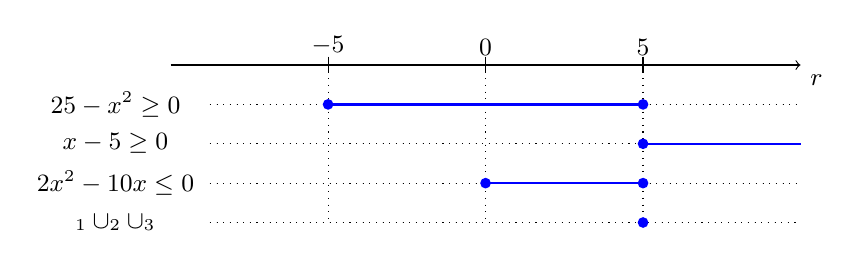
\begin{tikzpicture}[font=\small,x=10mm, y=10mm]
%IS1
\draw[->] (0,0) -- (8,0) node [below right] () {$r$};

\foreach \x in {2,4,6}{
\draw(\x,3pt)--(\x,-3pt);
\begin{scope}[dotted]
\draw (\x,0) -- (\x,-2);
\draw (.5,-.5) -- (2,-.5);
\draw (6,-.5) -- (8,-.5);
\draw (.5,-1) -- (6,-1);
\draw (.5,-1.5) -- (4,-1.5);
\draw (6,-1.5) -- (8,-1.5);
\draw (.5,-2) -- (8,-2);
\end{scope}}

\node[above]  at (2,0) {$-5$};
\node[above]  at (4,0) {$0$};
\node[above]  at (6,0) {$5$};
\node[] () at (-.7,-.5) {$25-x^2\ge 0$};
\node[] () at (-.7,-1) {$x-5\ge 0$};
\node[] () at (-.7,-1.5) {$2x^2-10x\le 0$};
\node[] () at (-.7,-2) {$\IS_1\cup\IS_2\cup\IS_3$};

\begin{scope}[blue,thick]
\draw (2,-.5) -- (6,-.5);
\draw (6,-1) -- (8,-1);
\draw (4,-1.5) -- (6,-1.5);
\draw[fill=blue] (2,-.5)circle (1.5pt);
\draw[fill=blue] (6,-.5)circle (1.5pt);
\draw[fill=blue] (6,-1)circle (1.5pt);
\draw[fill=blue] (4,-1.5)circle (1.5pt);
\draw[fill=blue] (6,-1.5)circle (1.5pt);
\draw[fill=blue] (6,-2)circle (1.5pt);
\end{scope}

\end{tikzpicture}

\end{center}

La disequazione è verificata solo per $x=5$.
\end{esempio}

\begin{esempio}
Risolvere la seguente disequazione irrazionale $\sqrt{x+3}<\sqrt{3x+1}$.

La disequazione è equivalente al sistema: 
\[\left\{\begin{array}{l}x+3\ge 0\\3x+1\ge 0\\x+3<3x+1\end{array}\right..\]

La prima disequazione indica le condizioni di esistenza del primo radicale, la seconda indica le condizione di esistenza del secondo radicale e dato che i due membri della disequazione sono positivi, la terza disequazione è quella data, nei quali entrambi i membri sono stati elevati al quadrato.

Eseguendo i vari passaggi si ha: \[\left\{\begin{array}{l}x+3\ge 0\\3x+1\ge 0\\x+3<3x+1\end{array}\right.\Rightarrow \left\{\begin{array}{l}x\ge -3\\x\ge -\frac 1 3\\x>1 \end{array}\right..\]

\begin{center}
 % (c) 2013 Claudio Carboncini - claudio.carboncini@gmail.com
\begin{tikzpicture}[font=\small,x=10mm, y=10mm]
%IS1
\draw[->] (0,0) -- (8,0) node [below right] () {$r$};

\foreach \x in {2,4,6}{
\draw(\x,3pt)--(\x,-3pt);
\begin{scope}[dotted]
\draw (\x,0) -- (\x,-2);
\draw (.5,-.5) -- (2,-.5);
\draw (.5,-1) -- (6,-1);
\draw (.5,-1.5) -- (6,-1.5);
\draw (.5,-2) -- (8,-2);
\end{scope}}
\node[above]  at (2,0) {$-3$};
\node[above]  at (4,0) {$-\frac 1 3$};
\node[above]  at (6,0) {$1$};
\pattern[pattern= north east lines, pattern color=Maroon] (6,-2.5) rectangle (8,-2);
\node[] () at (-.7,-.5) {$x+3\ge 0$};
\node[] () at (-.7,-1) {$3x+1\ge 0$};
\node[] () at (-.7,-1.5) {$x>1$};
\node[] () at (-.7,-2) {$\IS_1\cup\IS_2\cup\IS_3$};
\begin{scope}[blue,thick]
\draw (2,-.5) -- (8,-.5);
\draw (4,-1) -- (8,-1);
\draw (6,-1.5) -- (8,-1.5);
\draw[fill=blue] (2,-.5)circle (1.5pt);
\draw[fill=blue] (4,-1)circle (1.5pt);
\draw[fill=white] (6,-1.5)circle (1.5pt);
\draw[fill=white] (6,-2)circle (1.5pt);
\end{scope}

\end{tikzpicture}

\end{center}

La disequazione è verificata per $ x>1 $.
\end{esempio}
\end{exrig}

\ovalbox{\risolvii \ref{ese:8.19}, \ref{ese:8.20}, \ref{ese:8.21}, \ref{ese:8.22}, \ref{ese:8.23}, \ref{ese:8.24}, \ref{ese:8.25}, \ref{ese:8.26}}

\newpage
% (c)~2014 Claudio Carboncini - claudio.carboncini@gmail.com
% (c)~2014 Dimitrios Vrettos - d.vrettos@gmail.com
\section{Esercizi}
\subsection{Esercizi dei singoli paragrafi}
\subsection*{8.1 - Equazioni irrazionali con un solo radicale}
Risolvi le seguenti equazioni irrazionali con un radicale.
\begin{esercizio}[\Ast]
 \label{ese:8.1}
Risolvi le seguenti equazioni irrazionali con un radicale.
\begin{multicols}{2}
 \begin{enumeratea}
 \item~$\sqrt{2x+1}=7$;
 \item~$\sqrt{4-x^2}=1$;
 \item~$\sqrt[4]{2x+1}=2$;
 \item~$\sqrt[3]{2x+1}=-2$.
 \end{enumeratea}
 \end{multicols}
\end{esercizio}

\begin{esercizio}
 \label{ese:8.2}
Risolvi le seguenti equazioni irrazionali con un radicale.
\begin{multicols}{2}
 \begin{enumeratea}
 \item~$\sqrt[3]{x+1}=-1$;
 \item~$\sqrt[3]{x^2-6x}=3$;
 \item~$\sqrt{5x-2}=-4$;
 \item~$\sqrt{2-x^2+x}=6$.
 \end{enumeratea}
 \end{multicols}
\end{esercizio}

\begin{esercizio}[\Ast]
 \label{ese:8.3}
Risolvi le seguenti equazioni irrazionali con un radicale.
\begin{multicols}{2}
 \begin{enumeratea}
 \item~$\sqrt{2x^2+9}=2$;
 \item~$\sqrt[3]{16x-64}=x-4$;
 \item~$\sqrt{3x+10}=1-\frac 3 2x$;
 \item~$\sqrt[3]{3x+10}=1-\frac 3 2x$.
 \end{enumeratea}
 \end{multicols}
\end{esercizio}

\begin{esercizio}[\Ast]
 \label{ese:8.4}
Risolvi le seguenti equazioni irrazionali con un radicale.
\begin{multicols}{2}
 \begin{enumeratea}
 \item~$-3=\sqrt{\frac 2{x+1}}$;
 \item~$x-\sqrt{x+2}=0$;
 \item~$\sqrt[3]{3x+1-3x^2}=x$;
 \item~$\sqrt{25-x^2}+x=7$.
 \end{enumeratea}
 \end{multicols}
\end{esercizio}

\begin{esercizio}[\Ast]
 \label{ese:8.5}
Risolvi le seguenti equazioni irrazionali con un radicale.
\begin{multicols}{2}
 \begin{enumeratea}
 \item~$\sqrt{x^2+1}-3+x^2=(x-2)^2$;
 \item~$\sqrt{\frac{x-1}{3-x}}=\frac 1{x-3}$;
 \item~$\sqrt{\frac{2+3x} x}=\frac 1 x+1$;
 \item~$\sqrt{3x^2+10}=3x$.
 \end{enumeratea}
 \end{multicols}
\end{esercizio}

\begin{esercizio}[\Ast]
 \label{ese:8.6}
Risolvi le seguenti equazioni irrazionali con un radicale.
\begin{multicols}{2}
 \begin{enumeratea}
 \item~$\sqrt[3]{\frac{2x^2-1} x}-x=0$;
 \item~$\sqrt[2]{\frac{2x^2-1} x}-x=0$;
 \item~$\frac{4x+1}{2x}=\sqrt{\frac 2{x+1}}$;
 \item~$\sqrt{\frac{x-1}{3-x}}=\frac 1{x-3}$.
 \end{enumeratea}
 \end{multicols}
\end{esercizio}

\begin{esercizio}[\Ast]
 \label{ese:8.7}
Risolvi le seguenti equazioni irrazionali con un radicale.
\begin{multicols}{2}
 \begin{enumeratea}
 \item~$x\sqrt{x^2-4}=x^2-4$;
 \item~$\sqrt[3]{2x^2-7x+5}=1-x$;
 \item~$\frac{\sqrt{2x-3}}{x-2}=2$;
 \item~$\sqrt{4x-1}=\sqrt 2+\sqrt 3$.
 \end{enumeratea}
 \end{multicols}
\end{esercizio}
\pagebreak
\begin{esercizio}[\Ast]
 \label{ese:8.8}
Risolvi le seguenti equazioni irrazionali con un radicale.
\begin{multicols}{2}
 \begin{enumeratea}
 \item~$\sqrt{x+2}=x-1$;
 \item~$2\sqrt{x^2-4x-33}-x=15$;
 \item~$(3-x)^2-\sqrt{x-2x^2+5}=(x-3)(x-2)$;
 \item~$4x+\frac 1 2\sqrt{25-x^2}=\frac 7 2(x+1)$.
 \end{enumeratea}
 \end{multicols}
\end{esercizio}

\begin{esercizio}[\Ast]
 \label{ese:8.9}
Risolvi le seguenti equazioni irrazionali con un radicale.
\begin{multicols}{2}
 \begin{enumeratea}
 \item~$\frac 1 3\sqrt{5x^2+4x-8}+x=2\left(x-\frac 1 3\right)$;
 \item~$1-x+\sqrt{8x^2-21x+34}=-3+2x$;
 \item~$\sqrt[4]{\frac{(x-1)^3} x}\cdot \sqrt[4]{\frac{x^3}{x-1}}=x+\frac 3 2$.
 \end{enumeratea}
 \end{multicols}
\end{esercizio}

\subsection*{8.2 - Equazioni irrazionali con più radicali}

\begin{esercizio}[\Ast]
 \label{ese:8.10}
Risolvi le seguenti equazioni irrazionali con più radicali.
\begin{multicols}{2}
 \begin{enumeratea}
 \item~$\sqrt{3x-5}=\sqrt{1-x}$;
 \item~$\sqrt{3x-2}=\sqrt{2x-3}$;
 \item~$\sqrt{x-2}=1-\sqrt{3-x}$;
 \item~$\sqrt{6-3x}=2+\sqrt{x+1}$.
 \end{enumeratea}
 \end{multicols}
\end{esercizio}

\begin{esercizio}[\Ast]
 \label{ese:8.11}
Risolvi le seguenti equazioni irrazionali con più radicali.
\begin{multicols}{2}
 \begin{enumeratea}
 \item~$\sqrt{4-3x}=\sqrt{x^2-x-1}$;
 \item~$\sqrt{3-2x}=-\sqrt{x^2+3}$;
 \item~$\sqrt{3-x}=\sqrt{x+1}-1$;
 \item~$2\sqrt{x-1}=\sqrt{1+2x}+1$.
 \end{enumeratea}
 \end{multicols}
\end{esercizio}

\begin{esercizio}[\Ast]
 \label{ese:8.12}
Risolvi le seguenti equazioni irrazionali con più radicali.
\begin{multicols}{2}
 \begin{enumeratea}
 \item~$3\sqrt{x-x^2}=2\sqrt{x-1}$;
 \item~$\sqrt{x+1}=3\sqrt{4-x}$;
 \item~$\sqrt{x^2-x-3}=2\sqrt{x+5}$;
 \item~$1+2\sqrt{1-\frac 2 3x}=\sqrt{2x+1}$.
 \end{enumeratea}
 \end{multicols}
\end{esercizio}

\begin{esercizio}[\Ast]
 \label{ese:8.13}
Risolvi le seguenti equazioni irrazionali con più radicali.
\begin{multicols}{2}
 \begin{enumeratea}
 \item~$4-\sqrt{x-2}=\sqrt{x-1}+3$;
 \item~$2-2\sqrt{2-x}=4\sqrt{1-x}$;
 \item~$\sqrt{x^3-2x^2}=3\sqrt{x^2-2x}$;
 \item~$3\sqrt{x^4-x^3}=4\sqrt{x^4+2x^3}$.
 \end{enumeratea}
 \end{multicols}
\end{esercizio}

\begin{esercizio}[\Ast]
 \label{ese:8.14}
Risolvi le seguenti equazioni irrazionali con più radicali.
\begin{multicols}{2}
 \begin{enumeratea}
 \item~$\sqrt{2x^2-4x-3}=\sqrt{x^2-1}$;
 \item~$\sqrt{x^2+8}=\sqrt{4-x^2}$;
 \item~$\sqrt{x+12}-1=\sqrt{1-x}$;
 \item~$\sqrt{2x-5}=3-\sqrt{x+1}$.
 \end{enumeratea}
 \end{multicols}
\end{esercizio}

\begin{esercizio}[\Ast]
 \label{ese:8.15}
Risolvi le seguenti equazioni irrazionali con più radicali.
\begin{multicols}{2}
 \begin{enumeratea}
 \item~$\sqrt{x^2-2x+3}=\sqrt{1-x^2+2x}$;
 \item~$\sqrt{4x-7}+\sqrt{7x-4x^2}=0$;
 \item~$\sqrt{x^2+6x+9}+2\sqrt{1-x}=0$;
 \item~$\sqrt{2x+1}+\sqrt{x-2}=4$.
 \end{enumeratea}
 \end{multicols}
\end{esercizio}

\begin{esercizio}[\Ast]
 \label{ese:8.16}
Risolvi le seguenti equazioni irrazionali con più radicali.
\begin{multicols}{2}
 \begin{enumeratea}
 \item~$\sqrt{x^2-4}=3+2\sqrt{1-x^2}$;
 \item~$\sqrt{4+x^2}=1+\sqrt{x^2-1}$;
 \item~$\sqrt{2x+1}=3+2\sqrt{x-6}$;
 \item~$\sqrt{x-2}-\sqrt{2x-1}=\sqrt{5x-1}$.
 \end{enumeratea}
 \end{multicols}
\end{esercizio}
\pagebreak
\begin{esercizio}[\Ast]
 \label{ese:8.17}
Risolvi le seguenti equazioni irrazionali con più radicali.
\begin{multicols}{2}
 \begin{enumeratea}
 \item~$\sqrt{4-x}+2\sqrt{x}=0$;
 \item~$\sqrt{16+x}-\sqrt{x}=\sqrt{x-5}$;
 \item~$5-\sqrt[3]{2(x-1)}=\sqrt[3]{37-2x}$;
 \item~$\sqrt{x-1}=\sqrt{x+1-\sqrt{x-1}}$.
 \end{enumeratea}
 \end{multicols}
\end{esercizio}

\begin{esercizio}[\Ast]
 \label{ese:8.18}
Risolvi le seguenti equazioni irrazionali con più radicali.
\begin{multicols}{2}
 \begin{enumeratea}
 \item~$\sqrt{\frac{(3-2x)}{(x-1)}}+\sqrt{2x-1}=\sqrt{\frac 1{x-1}}$;
 \item~$\sqrt{(x-1)^2+\sqrt{5x-6}}=2-x$;
 \item~$\frac{\sqrt{x-1}}{\sqrt{x+1}}=\sqrt{x-1}$;
 \item~$\sqrt{\frac x{4-x}}+3\sqrt{\frac{4-x} x}-4=0$;
 \item~$\frac 5{6-\sqrt x}+\frac 1 2=\frac 6{5-\sqrt x}$.
 \end{enumeratea}
 \end{multicols}
\end{esercizio}

\subsection*{8.3 - Disequazioni irrazionali}

\begin{esercizio}[\Ast]
 \label{ese:8.19}
Risolvi le seguenti disequazioni irrazionali.
\begin{multicols}{2}
 \begin{enumeratea}
 \item~$\sqrt{4x^2-x}\ge -2x+1$;
 \item~$\sqrt{x^2-x-2}\le 2x+6$;
 \item~$\sqrt{2x-1}\ge x-8$;
 \item~$\sqrt{x^2-3x+2}<7-5x$.
 \end{enumeratea}
 \end{multicols}
\end{esercizio}

\begin{esercizio}[\Ast]
 \label{ese:8.20}
Risolvi le seguenti disequazioni irrazionali.
\begin{multicols}{2}
 \begin{enumeratea}
 \item~$\sqrt{9x^2+2x}\ge 3x-4$;
 \item~$\sqrt{x^2-2x}\ge 5-x$;
 \item~$\sqrt{16-2x^2}<x+4$;
 \item~$\sqrt{3-2x}\le \sqrt{1-x^2}$.
 \end{enumeratea}
 \end{multicols}
\end{esercizio}

\begin{esercizio}[\Ast]
 \label{ese:8.21}
Risolvi le seguenti disequazioni irrazionali.
\begin{multicols}{2}
 \begin{enumeratea}
 \item~$\sqrt{4x^2+2x}\ge 2x-3$;
 \item~$\sqrt{1-x^2}>2x-1$;
 \item~$\sqrt{2x^2-x-1}>\sqrt{x-3}$;
 \item~$\sqrt{x^2+2x+1}\le \sqrt{1-x^2}$.
 \end{enumeratea}
 \end{multicols}
\end{esercizio}

\begin{esercizio}[\Ast]
 \label{ese:8.22}
Risolvi le seguenti disequazioni irrazionali.
\begin{multicols}{2}
 \begin{enumeratea}
 \item~$\sqrt{16x^2+2x}\ge -4x-1$;
 \item~$\sqrt{x^2-1}<x+3$;
 \item~$\sqrt{x^2-3x+2}\le \sqrt{3x^2-2x-1}$;
 \item~$\sqrt{9x^2-x}\ge -3x+6$.
 \end{enumeratea}
 \end{multicols}
\end{esercizio}

\begin{esercizio}[\Ast]
 \label{ese:8.23}
Risolvi le seguenti disequazioni irrazionali.
\begin{multicols}{2}
 \begin{enumeratea}
 \item~$\sqrt{x^2+1}\le \frac{x+\sqrt 3} 2$;
 \item~$\sqrt{x^2-5x}\ge x-4$;
 \item~$\sqrt{x^2+1}\le \frac 1 2x+1$;
 \item~$\sqrt{10x-x^2}>\sqrt{2x^2-32}$.
 \end{enumeratea}
 \end{multicols}
\end{esercizio}

\begin{esercizio}[\Ast]
 \label{ese:8.24}
Risolvi le seguenti disequazioni irrazionali.
\begin{multicols}{2}
 \begin{enumeratea}
 \item~$\sqrt{x^2+x}\ge x+3$;
 \item~$\sqrt{x^2+1}\le \frac 1 2x-1$;
 \item~$\sqrt{x^2+1}\le \sqrt{1-x^2}$;
 \item~$\sqrt{2x^2+x}\ge \sqrt{4-x^2}$.
 \end{enumeratea}
 \end{multicols}
\end{esercizio}
\pagebreak
\begin{esercizio}[\Ast]
 \label{ese:8.25}
Risolvi le seguenti disequazioni irrazionali.
\begin{multicols}{2}
 \begin{enumeratea}
 \item~$3\sqrt{3x+x^2}<2\sqrt{2x-x^3}$;
 \item~$2\sqrt{x+x^3}>\sqrt{2x^3-3x^2}$;
 \item~$\sqrt{x^5-x^3}<2\sqrt{x^4+2x^3}$.
 \end{enumeratea}
 \end{multicols}
\end{esercizio}

\begin{esercizio}[\Ast]
 \label{ese:8.26}
Risolvi le seguenti disequazioni irrazionali.
\begin{multicols}{2}
 \begin{enumeratea}
 \item~$\sqrt{3-2x}\le \sqrt{1+x^{2}}$;
 \item~$\sqrt{\frac{x^2-1}{2+x}}< \sqrt{x}$;
 \item~$\frac{1}{\sqrt{4-x^{2}}}\ge \frac{1}{x}$;
 \item~$\sqrt{\left|\frac{x+1}{x-1}\right|}> 1$.
 \end{enumeratea}
 \end{multicols}
\end{esercizio}

\subsection{Risposte}
%\begin{multicols}{2}
\paragraph{8.1.} a)~$x=24$,\quad b)~$x_{1\text{,}2}=\pm \sqrt 3$,\quad c)~$x=\frac{15} 2$,\quad d)~$x=-\frac 9 2$.

\paragraph{8.2.} a)~$x=-2$,\quad b)~$x_1=-3\vee x_2=9$,\quad c)~$\emptyset $,\quad d)~$\emptyset$.

\paragraph{8.3.} a)~$\emptyset$,\quad b)~$x_1=4\vee x_2=8$,\quad c)~$x=\frac{4-2\sqrt{13}} 3$,\quad d)~$x=-\frac 2 3$.

\paragraph{8.4.} a)~$\emptyset$,\quad b)~$x=2$,\quad c)~ $x=1$,\quad d)~$x_1=3\vee x_2=4$.

\paragraph{8.5.} a)~$x_1=\frac 4 3$,\quad b)~$\emptyset$,\quad c)~$x=\frac{\sqrt 2} 2$,\quad d)~$x=\frac{\sqrt{15}} 3$.

\paragraph{8.6.} a)~$x_1=-1\vee x_2=1$,\quad b)~$x_1=1\vee x_2=\frac{\sqrt 5+1} 2$,\quad c)~$\emptyset$,\quad d)~$\emptyset$.

\paragraph{8.7.} a)~$x_{1\text{,}2}=\mp 2$,\quad b)~$x_1=1\vee x_2=-2\vee x_3=2$,\quad c)~$x=\frac{9+\sqrt 5} 4$,\quad d)~$x=\frac{3+\sqrt 6} 2$.

\paragraph{8.8.} a)~$x=\frac{3+\sqrt{13}} 2$,\quad b)~$x_1=21\vee x_2=-\frac{17} 3$,\quad c)~$x_1=1\vee x_2=\frac 4 3$,\quad d)~$x_1=3\vee x_2=4$.

\paragraph{8.9.} a)~$x_1=1\vee x_2=3$,\quad b)~$x=6$,\quad c)~$x=-\frac 9{16}$.

\paragraph{8.10.} a)~$x=\frac 3 2$ non acc,\quad b)~$x=-1$ non acc,\quad c)~$x_1=2\vee x_2=3$,\quad d)~$x=\frac{3-2\sqrt 6} 4$.

\paragraph{8.11.} a)~$x=-1-\sqrt 6$,\quad b)~$\emptyset $,\quad c)~$x=\frac{2+\sqrt 7} 2$,\quad d)~$x=4+2\sqrt 2$.

\paragraph{8.12.} a)~$x=1$,\quad b)~$x=\frac 7 2$,\quad c)~$x_{1\text{,}2}=\frac{5\pm 3\sqrt{13}} 2$,\quad d)~$x=\frac{60}{49}$.

\paragraph{8.13.} a)~$x=2$,\quad b)~$x=1$,\quad c)~$x_1=0\vee x_2=2\vee x_3=9$,\quad d)~$x_1=0\vee x_2=-\frac{41} 7$.

\paragraph{8.14.} a)~$x=2+\sqrt 6$,\quad b)~$\emptyset $,\quad c)~$x=-3$,\quad d)~$x=3$.

\paragraph{8.15.} a)~$x=1$,\quad b)~$x=\frac{7}{4}$,\quad c)~$\emptyset$,\quad d)~$x=45-24\sqrt{3}$.

\paragraph{8.16.} a)~$\emptyset $,\quad b)~$x_{1\text{,}2}=\pm \sqrt 5$,\quad c)~$x=26-6\sqrt{11}$,\quad d)~$x=\frac{7-3\sqrt 5} 2$.

\paragraph{8.17.} a)~$\emptyset$,\quad b)~$x=9$,\quad c)~$x_1=5\vee x_2=\frac{29}{2}$,\quad d)~$x=5$.

\paragraph{8.18.} a)~$x=\frac 3 2$,\quad b)~$x=\frac 5 4$,\quad c)~$x=1$,\quad d)~$x_1=2\vee x_2=\frac{18} 5$,\quad e)~$x_1=1\vee x_2=64$.

\paragraph{8.19.} a)~$x\ge \frac 1 3$,\quad b)~$-2\le x\le -1\vee x\ge 2$,\quad c)~$\frac 1 2\le x\le 13$,\quad d)~$x\le 1$.

\paragraph{8.20.} a)~$x\le -\frac 2 9\vee x\ge 0$,\quad b)~$x\ge \frac{25} 8$,\quad c)~$-2\sqrt 2\le x<-\frac 8 3\vee 0<x\le 2\sqrt 2$,\quad d)~$ \emptyset $.

\paragraph{8.21.} a)~$x\le -\frac 1 2\vee x\ge 0$,\quad b)~$-1\le x<\frac 4 5$,\quad c)~$x\ge 3$,\quad d)~$-1\le x\le 0$.

\paragraph{8.22.} a)~$x\le -\frac 1 8\vee x\ge 0$,\quad b)~$-\frac 5 3<x\le -1\vee x\ge 1$,\quad c)~$x\le -\frac 3 2\vee x=1\vee x\ge 2$,\quad d)~$x\ge \frac{36}{35}$.

\paragraph{8.23.} a)~$x=\frac{\sqrt 3} 3$,\quad b)~$x\le 0\vee x\ge \frac{16} 3$,\quad c)~$0\le x\le \frac 4 3$,\quad d)~$4\le x<\frac{16} 3$.

\paragraph{8.24.} a)~$x\le -\frac 9 5$,\quad b)~$ \emptyset $,\quad c)~$x=0$,\quad d)~$-2\le x\le -\frac 4 3\vee 1\le x\le 2$.

\paragraph{8.25.} a)~$x\le -3$,\quad b)~$x\ge \frac 3 2$,\quad c)~$1\le x<2+\sqrt{13}$.

\paragraph{8.26.} a)~$x\le-1-\sqrt{3}\vee \sqrt{3}-1\le x\le \frac{3}{2}$,\quad b)~$x\ge 1$,\quad c)~$-2<x<0\vee \sqrt{2}\le x<2$,\quad d)~$x>0 \wedge x\neq 1$.
%\end{multicols}
\cleardoublepage
